% answers.tex —— 2018 年·浙江卷 · 参考答案与详细解析片段
% 由 tools/generate_projects.py 依来源总账自 2018/2018_数学真题_浙江_试题.md + 2018/2018_数学真题_浙江_解析正文.md + 2018/2018_数学真题_浙江_答案要点.md 生成，勿手改（改源 MD 后重跑）

\begin{gktip}
固定源没有答案页；以下为非官方推导，不能称为官方答案。
\end{gktip}

\gkpart{一、选择题}

\begin{answer}
\gksolhead{1}{}

\textbf{题目}：

已知全集 $U = \{1, 2, 3, 4, 5\}$，$A = \{1, 3\}$，则 $\complement_U A =$（ ）。

(A) $\varnothing$　(B) $\{1, 3\}$　(C) $\{2, 4, 5\}$　(D) $\{1, 2, 3, 4, 5\}$

\Needspace{4\baselineskip}
\textbf{解析}

全集 $U = \{1, 2, 3, 4, 5\}$，集合 $A = \{1, 3\}$。
\Needspace{5\baselineskip}
由补集定义可知，$\complement_U A$ 是由属于全集 $U$ 但不属于集合 $A$ 的所有元素构成的集合：
\nopagebreak[4]
\[\complement_U A = \{2, 4, 5\}.\]
故选 \textbf{C}。

\gkanswer{答案：C}

\end{answer}
\begin{answer}
\gksolhead{2}{}

\textbf{题目}：

双曲线 $\dfrac{x^2}{3} - y^2 = 1$ 的焦点坐标是（ ）。

(A) $(-\sqrt2, 0), (\sqrt2, 0)$　(B) $(-2, 0), (2, 0)$　(C) $(0, -\sqrt2), (0, \sqrt2)$　(D) $(0, -2), (0, 2)$

\Needspace{4\baselineskip}
\textbf{解析}

双曲线的标准方程为 $\dfrac{x^2}{3} - y^2 = 1$，焦点在 $x$ 轴上。
其中 $a^2 = 3$，$b^2 = 1$。
\Needspace{5\baselineskip}
由双曲线几何性质可知：
\nopagebreak[4]
\[c = \sqrt{a^2 + b^2} = \sqrt{3 + 1} = 2.\]
因此，双曲线的焦点坐标为 $(-2, 0)$ 和 $(2, 0)$。
故选 \textbf{B}。

\gkanswer{答案：B}

\end{answer}
\begin{answer}
\gksolhead{3}{}

\textbf{题目}：

某几何体的三视图如图所示（单位：$\mathrm{cm}$），则该几何体的体积（单位：$\mathrm{cm}^3$）是（ ）。
\nopagebreak[4]
\begin{center}% 2018 浙江卷第3题：三视图
\begin{tikzpicture}[font=\small, line cap=round, line join=round, >=stealth]
  % 正视图
  \begin{scope}
    \draw[thick] (0, 0) rectangle (2, 2);
    \draw[thick] (1, 0) -- (1, 2);
    % 尺寸标注
    \draw[<->] (0, -0.2) -- (1, -0.2) node[midway, fill=white, inner sep=1pt] {$1$};
    \draw[<->] (1, -0.2) -- (2, -0.2) node[midway, fill=white, inner sep=1pt] {$1$};
    \draw[<->] (2.2, 0) -- (2.2, 2) node[midway, fill=white, inner sep=1pt] {$2$};
    \node[below=5mm] at (1, 0) {正视图};
  \end{scope}

  % 侧视图
  \begin{scope}[xshift=3.2cm]
    \draw[thick] (0, 0) rectangle (2, 2);
    % 尺寸标注
    \draw[<->] (0, -0.2) -- (2, -0.2) node[midway, fill=white, inner sep=1pt] {$2$};
    \node[below=5mm] at (1, 0) {侧视图};
  \end{scope}

  % 俯视图（位于正视图下方）
  \begin{scope}[yshift=-3.4cm]
    \draw[thick] (0, 2) -- (2, 2) -- (2, 0) -- (1, 0) -- cycle;
    \node[below=3mm] at (1, 0) {俯视图};
  \end{scope}
\end{tikzpicture}
\end{center}
\nopagebreak[4]
(A) $2$　(B) $4$　(C) $6$　(D) $8$

\Needspace{4\baselineskip}
\textbf{解析}

由三视图可知：
该几何体是一个以俯视图为底面的直四棱柱。
底面为一个直角梯形，其上底为 $2$，下底为 $1$，高为 $2$。
\Needspace{5\baselineskip}
底面直角梯形的面积为：
\nopagebreak[4]
\[S = \dfrac{2 + 1}{2} \times 2 = 3\ (\mathrm{cm}^2).\]
由正视图与侧视图可知，直四棱柱的高为 $h = 2\ \mathrm{cm}$。
\Needspace{5\baselineskip}
因此，该几何体的体积为：
\nopagebreak[4]
\[V = S \times h = 3 \times 2 = 6\ (\mathrm{cm}^3).\]
故选 \textbf{C}。

\gkanswer{答案：C}

\end{answer}
\begin{answer}
\gksolhead{4}{}

\textbf{题目}：

复数 $\dfrac{2}{1 - \mathrm i}$（$\mathrm i$ 为虚数单位）的共轭复数是（ ）。

(A) $1 + \mathrm i$　(B) $1 - \mathrm i$　(C) $-1 + \mathrm i$　(D) $-1 - \mathrm i$

\Needspace{4\baselineskip}
\textbf{解析}

\Needspace{5\baselineskip}
化简复数：
\nopagebreak[4]
\[\dfrac{2}{1 - \mathrm i} = \dfrac{2(1 + \mathrm i)}{(1 - \mathrm i)(1 + \mathrm i)} = \dfrac{2(1 + \mathrm i)}{1 - \mathrm i^2} = \dfrac{2(1 + \mathrm i)}{2} = 1 + \mathrm i.\]
根据共轭复数的定义，实部不变、虚部互为相反数，故其共轭复数为 $1 - \mathrm i$。
故选 \textbf{B}。

\gkanswer{答案：B}

\end{answer}
\begin{answer}
\gksolhead{5}{}

\textbf{题目}：

函数 $y = 2^{|x|}\sin 2x$ 的图象可能是（ ）。
\nopagebreak[4]
\begin{center}% 2018 浙江卷第5题：函数图象选项
\begin{tikzpicture}[line cap=round, line join=round, line width=0.6pt, font=\small]

% (A) 偶函数图象
\begin{scope}[shift={(0, 3.2)}, x=0.8cm, y=0.5cm]
  \draw[->] (-3.8, 0) -- (3.8, 0) node[below] {$x$};
  \draw[->] (0, -2.2) -- (0, 3.2) node[left] {$y$};
  \node[below right] at (0, 0) {$O$};
  \draw (-3.14, 0.08) -- (-3.14, -0.08) node[below left] {$-\pi$};
  \draw (3.14, 0.08) -- (3.14, -0.08) node[below right] {$\pi$};
  \begin{scope}
    \clip (-3.6, -2.0) rectangle (3.6, 3.0);
    \draw[thick, domain=-3.5:3.5, samples=120] plot (\x, {2.2 * sin(deg(abs(\x)))});
  \end{scope}
  \node at (0, -2.7) {(A)};
\end{scope}

% (B) 偶函数双峰双谷图象
\begin{scope}[shift={(6.8, 3.2)}, x=0.8cm, y=0.5cm]
  \draw[->] (-3.8, 0) -- (3.8, 0) node[below] {$x$};
  \draw[->] (0, -2.6) -- (0, 3.2) node[left] {$y$};
  \node[below right] at (0, 0) {$O$};
  \draw (-3.14, 0.08) -- (-3.14, -0.08) node[below left] {$-\pi$};
  \draw (3.14, 0.08) -- (3.14, -0.08) node[below right] {$\pi$};
  \begin{scope}
    \clip (-3.6, -2.4) rectangle (3.6, 3.0);
    \draw[thick, domain=-3.5:3.5, samples=120] plot (\x, {1.2 * cos(2*deg(\x)) - 1.2 * abs(\x)/3.14 + 0.3});
  \end{scope}
  \node at (0, -2.7) {(B)};
\end{scope}

% (C) 奇函数单正峰单负谷图象
\begin{scope}[shift={(0, -3.2)}, x=0.8cm, y=0.5cm]
  \draw[->] (-3.8, 0) -- (3.8, 0) node[below] {$x$};
  \draw[->] (0, -2.6) -- (0, 3.2) node[left] {$y$};
  \node[below right] at (0, 0) {$O$};
  \draw (-3.14, 0.08) -- (-3.14, -0.08) node[below left] {$-\pi$};
  \draw (3.14, 0.08) -- (3.14, -0.08) node[below right] {$\pi$};
  \begin{scope}
    \clip (-3.6, -2.4) rectangle (3.6, 3.0);
    \draw[thick, domain=-3.5:3.5, samples=100] plot (\x, {2.0 * sin(deg(\x))});
  \end{scope}
  \node at (0, -2.7) {(C)};
\end{scope}

% (D) 正确选项：y = 2^{|x|} \sin 2x
\begin{scope}[shift={(6.8, -3.2)}, x=0.8cm, y=0.5cm]
  \draw[->] (-3.8, 0) -- (3.8, 0) node[below] {$x$};
  \draw[->] (0, -2.8) -- (0, 3.2) node[left] {$y$};
  \node[below right] at (0, 0) {$O$};
  \draw (-3.14, 0.08) -- (-3.14, -0.08) node[below left] {$-\pi$};
  \draw (3.14, 0.08) -- (3.14, -0.08) node[below right] {$\pi$};
  \begin{scope}
    \clip (-3.6, -2.6) rectangle (3.6, 2.8);
    \draw[thick, domain=-3.4:3.4, samples=140] plot (\x, {0.35 * pow(2, abs(\x)) * sin(2*deg(\x))});
  \end{scope}
  \node at (0, -2.7) {(D)};
\end{scope}

\end{tikzpicture}
\end{center}
\nopagebreak[4]
(A) 见图 (A)　(B) 见图 (B)　(C) 见图 (C)　(D) 见图 (D)

\Needspace{4\baselineskip}
\textbf{解析}

考察函数 $f(x) = 2^{|x|}\sin 2x$ 的性质：
\Needspace{5\baselineskip}
1. \textbf{奇偶性}：定义域为 $\mathbf R$，关于原点对称。
\nopagebreak[4]
\[f(-x) = 2^{|-x|}\sin(-2x) = 2^{|x|}(-\sin 2x) = -f(x).\]
   所以函数 $f(x)$ 为奇函数，其图象关于原点对称，排除选项 A、B。
2. \textbf{函数值符号}：
   当 $x \in \left(0, \dfrac\pi2\right)$ 时，$2x \in (0, \pi)$，$\sin 2x > 0$，又 $2^{|x|} > 0$，故 $f(x) > 0$；
   当 $x \in \left(\dfrac\pi2, \pi\right)$ 时，$2x \in (\pi, 2\pi)$，$\sin 2x < 0$，故 $f(x) < 0$。
   选项 C 在 $(0, \pi)$ 上全为正值，不符合题意，排除选项 C。
3. \textbf{振幅特征}：
   随着 $|x|$ 增大，振幅放大因子 $2^{|x|}$ 严格单调递增，波谷深度明显大于先前的波峰高度，选项 D 图象完全符合该特征。
故选 \textbf{D}。

\gkanswer{答案：D}

\end{answer}
\begin{answer}
\gksolhead{6}{}

\textbf{题目}：

已知平面 $\alpha$，直线 $m, n$ 满足 $m \not\subset \alpha$，$n \subset \alpha$，则“$m \parallel n$”是“$m \parallel \alpha$”的（ ）。

(A) 充分不必要条件　(B) 必要不充分条件　(C) 充分必要条件　(D) 既不充分也不必要条件

\Needspace{4\baselineskip}
\textbf{解析}

已知平面 $\alpha$，直线 $m, n$ 满足 $m \not\subset \alpha$，$n \subset \alpha$。
1. \textbf{充分性}：若 $m \parallel n$，由线面平行的判定定理（若平面外一条直线平行于平面内的一条直线，则该直线平行于此平面），可知 $m \parallel \alpha$ 成立，故充分性成立；
2. \textbf{必要性}：若 $m \parallel \alpha$，且 $n \subset \alpha$，直线 $m$ 与平面 $\alpha$ 无公共点，因此 $m$ 与 $n$ 既没有公共点，又可能在同一平面内（平行），也可能不在同一平面内（异面）。故不能推出 $m \parallel n$，必要性不成立。
综上，“$m \parallel n$”是“$m \parallel \alpha$”的充分不必要条件。
故选 \textbf{A}。

\gkanswer{答案：A}

\end{answer}
\begin{answer}
\gksolhead{7}{}

\textbf{题目}：

\Needspace{5\baselineskip}
设 $0 < p < 1$，随机变量 $\xi$ 的分布列是

\nopagebreak[4]
\[\begin{array}{|c|c|c|c|}
\hline
\xi & 0 & 1 & 2 \\
\hline
P & \dfrac{1-p}{2} & \dfrac12 & \dfrac{p}{2} \\
\hline
\end{array}\]

则当 $p$ 在 $(0, 1)$ 内增大时，（ ）。

(A) $D(\xi)$ 减小　(B) $D(\xi)$ 增大　(C) $D(\xi)$ 先减小后增大　(D) $D(\xi)$ 先增大后减小

\Needspace{4\baselineskip}
\textbf{解析}

\Needspace{5\baselineskip}
随机变量 $\xi$ 的分布列为离散型分布，概率之和满足：
\nopagebreak[4]
\[\dfrac{1-p}{2} + \dfrac12 + \dfrac{p}{2} = 1.\]
\Needspace{5\baselineskip}
计算数学期望：
\nopagebreak[4]
\[E(\xi) = 0 \times \dfrac{1-p}{2} + 1 \times \dfrac12 + 2 \times \dfrac{p}{2} = \dfrac12 + p = p + \dfrac12.\]
\Needspace{5\baselineskip}
计算二阶原点矩：
\nopagebreak[4]
\[E(\xi^2) = 0^2 \times \dfrac{1-p}{2} + 1^2 \times \dfrac12 + 2^2 \times \dfrac{p}{2} = \dfrac12 + 2p.\]
\Needspace{5\baselineskip}
计算方差：
\nopagebreak[4]
\[\begin{aligned}
D(\xi) &= E(\xi^2) - [E(\xi)]^2 \\
&= \dfrac12 + 2p - \left(p + \dfrac12\right)^2 \\
&= \dfrac12 + 2p - \left(p^2 + p + \dfrac14\right) \\
&= -p^2 + p + \dfrac14 \\
&= -\left(p - \dfrac12\right)^2 + \dfrac12.
\end{aligned}\]
考察二次函数 $D(\xi) = -\left(p - \dfrac12\right)^2 + \dfrac12$，开口向下，对称轴为 $p = \dfrac12$。
当 $p$ 在区间 $(0, 1)$ 内逐渐增大时：
在 $\left(0, \dfrac12\right)$ 上，$D(\xi)$ 单调递增；在 $\left(\dfrac12, 1\right)$ 上，$D(\xi)$ 单调递减。
因此，$D(\xi)$ 先增大后减小。
故选 \textbf{D}。

\gkanswer{答案：D}

\end{answer}
\begin{answer}
\gksolhead{8}{}

\textbf{题目}：

已知四棱锥 $S - ABCD$ 的底面是正方形，侧棱长均相等，$E$ 是线段 $AB$ 上的点（不含端点），设 $SE$ 与 $BC$ 所成的角为 $\theta_1$，$SE$ 与平面 $ABCD$ 所成的角为 $\theta_2$，二面角 $S - AB - C$ 的平面角为 $\theta_3$，则（ ）。

(A) $\theta_1 \leqslant \theta_2 \leqslant \theta_3$　(B) $\theta_3 \leqslant \theta_2 \leqslant \theta_1$　(C) $\theta_1 \leqslant \theta_3 \leqslant \theta_2$　(D) $\theta_2 \leqslant \theta_3 \leqslant \theta_1$

\Needspace{4\baselineskip}
\textbf{解析}

设正方形底面边长为 $2a$，中心为 $O$。
由正四棱锥性质可知，$SO \perp$ 底面 $ABCD$，设高 $SO = h$。
取线段 $AB$ 的中点 $M$，则 $OM \perp AB$ 且 $OM = a$。
因为 $SO \perp$ 底面 $ABCD$，$OM \perp AB$，所以由三垂线定理知 $SM \perp AB$。
\Needspace{5\baselineskip}
因此，二面角 $S - AB - C$ 的平面角为 $\theta_3 = \angle SMO$，满足：
\nopagebreak[4]
\[\tan\theta_3 = \dfrac{SO}{OM} = \dfrac{h}{a},\quad \cos\theta_3 = \dfrac{a}{\sqrt{a^2 + h^2}}.\]
设点 $E$ 在线段 $AB$ 上（不含端点），在底面内过 $E$ 作底面高线 $EF \perp CD$（即 $EF \parallel BC$）。
因为 $AD \parallel BC$，所以 $SE$ 与 $BC$ 所成的角 $\theta_1$ 等于 $SE$ 与 $EF$ 所成的角。
以 $O$ 为原点建立空间直角坐标系，设 $A(-a, -a, 0)$，$B(a, -a, 0)$，$S(0, 0, h)$。
则 $\overrightarrow{BC}$ 的方向向量为 $(0, 1, 0)$。
设 $E(x_0, -a, 0)$，其中 $x_0 \in (-a, a)$。
则 $\overrightarrow{SE} = (x_0, -a, -h)$，$|\overrightarrow{SE}| = \sqrt{x_0^2 + a^2 + h^2}$。
\Needspace{5\baselineskip}
1. \textbf{分析 $\theta_1$ 与 $\theta_3$}：
\nopagebreak[4]
\[\cos\theta_1 = \dfrac{|\overrightarrow{SE} \cdot (0, 1, 0)|}{|\overrightarrow{SE}|} = \dfrac{a}{\sqrt{x_0^2 + a^2 + h^2}}.\]
\Needspace{5\baselineskip}
   因为 $x_0^2 \geqslant 0$，所以：
\nopagebreak[4]
\[\sqrt{x_0^2 + a^2 + h^2} \geqslant \sqrt{a^2 + h^2} \implies \cos\theta_1 \leqslant \cos\theta_3.\]
\Needspace{5\baselineskip}
   由于 $\theta_1, \theta_3 \in \left(0, \dfrac\pi2\right)$，余弦函数在该区间上单调递减，因此：
\nopagebreak[4]
\[\theta_3 \leqslant \theta_1.\]
2. \textbf{分析 $\theta_2$ 与 $\theta_3$}：
   直线 $SE$ 与平面 $ABCD$ 所成的角为 $\theta_2 = \angle SEO$。
   在 Rt$\triangle SOE$ 中，$\tan\theta_2 = \dfrac{SO}{OE} = \dfrac{h}{OE}$。
   在底面正方形中，$OE = \sqrt{x_0^2 + a^2} \geqslant a = OM$。
\Needspace{5\baselineskip}
   所以：
\nopagebreak[4]
\[\tan\theta_2 = \dfrac{h}{OE} \leqslant \dfrac{h}{a} = \tan\theta_3.\]
\Needspace{5\baselineskip}
   由于正切函数在 $\left(0, \dfrac\pi2\right)$ 上单调递增，因此：
\nopagebreak[4]
\[\theta_2 \leqslant \theta_3.\]
\Needspace{5\baselineskip}
综合上述两方面，可得：
\nopagebreak[4]
\[\theta_2 \leqslant \theta_3 \leqslant \theta_1.\]
故选 \textbf{D}。

\gkanswer{答案：D}

\end{answer}
\begin{answer}
\gksolhead{9}{}

\textbf{题目}：

已知 $\boldsymbol a, \boldsymbol b, \boldsymbol e$ 是平面向量，$\boldsymbol e$ 是单位向量。若非零向量 $\boldsymbol a$ 与 $\boldsymbol e$ 的夹角为 $\dfrac{\pi}{3}$，向量 $\boldsymbol b$ 满足 $\boldsymbol b^2 - 4\boldsymbol e \cdot \boldsymbol b + 3 = 0$，则 $|\boldsymbol a - \boldsymbol b|$ 的最小值是（ ）。

(A) $\sqrt3 - 1$　(B) $\sqrt3 + 1$　(C) $2$　(D) $2 - \sqrt3$

\Needspace{4\baselineskip}
\textbf{解析}

设 $\boldsymbol e$ 的方向为 $x$ 轴正方向，建立平面直角坐标系，则单位向量 $\boldsymbol e = (1, 0)$。
\Needspace{5\baselineskip}
对向量 $\boldsymbol b$ 的模方程配方：
\nopagebreak[4]
\[\boldsymbol b^2 - 4\boldsymbol e \cdot \boldsymbol b + 3 = 0 \iff |\boldsymbol b - 2\boldsymbol e|^2 = 4|\boldsymbol e|^2 - 3 = 1.\]
因此，向量 $\boldsymbol b$ 的终点 $B$ 在以点 $C_0(2, 0)$ 为圆心、半径为 $R = 1$ 的圆上。
非零向量 $\boldsymbol a$ 与 $\boldsymbol e$ 的夹角为 $\dfrac\pi3$，故向量 $\boldsymbol a$ 的终点 $A$ 落在从原点出发、倾斜角为 $60^\circ$ 的射线 $l\colon y = \sqrt3 x\ (x > 0)$ 上。
由平面几何性质，$|\boldsymbol a - \boldsymbol b|$ 表示圆 $C_0$ 上的动点 $B$ 到射线 $l$ 上的动点 $A$ 的欧氏距离。
\Needspace{5\baselineskip}
圆心 $C_0(2, 0)$ 到直线 $\sqrt3 x - y = 0$ 的距离为：
\nopagebreak[4]
\[d = \dfrac{|\sqrt3 \times 2 - 0|}{\sqrt{(\sqrt3)^2 + (-1)^2}} = \dfrac{2\sqrt3}{2} = \sqrt3.\]
圆心向直线作垂线，垂足的横坐标 $x > 0$，落在射线 $l$ 上。
\Needspace{5\baselineskip}
因此，$|\boldsymbol a - \boldsymbol b|$ 的最小值为圆上点到直线的最近距离：
\nopagebreak[4]
\[|\boldsymbol a - \boldsymbol b|_{\min} = d - R = \sqrt3 - 1.\]
故选 \textbf{A}。

\gkanswer{答案：A}

\end{answer}
\begin{answer}
\gksolhead{10}{}

\textbf{题目}：

已知 $a_1, a_2, a_3, a_4$ 成等比数列，且 $a_1 + a_2 + a_3 + a_4 = \ln(a_1 + a_2 + a_3)$。若 $a_1 > 1$，则（ ）。

(A) $a_1 < a_3, a_2 < a_4$　(B) $a_1 > a_3, a_2 < a_4$　(C) $a_1 < a_3, a_2 > a_4$　(D) $a_1 > a_3, a_2 > a_4$

\Needspace{4\baselineskip}
\textbf{解析}

设等比数列 $\{a_n\}$ 的公比为 $q$。
则 $a_2 = a_1 q$，$a_3 = a_1 q^2$，$a_4 = a_1 q^3$。
\Needspace{5\baselineskip}
已知：
\nopagebreak[4]
\[a_1(1 + q + q^2 + q^3) = \ln[a_1(1 + q + q^2)].\]
记 $S_3 = a_1(1 + q + q^2)$，$S_4 = a_1(1 + q + q^2 + q^3) = S_3 + a_4$。
1. \textbf{确定公比 $q$ 的符号与范围}：
\begin{itemize}
\item 因为 $a_1 > 1 > 0$，且 $1 + q + q^2 = \left(q + \dfrac12\right)^2 + \dfrac34 > 0$，所以 $S_3 > 0$ 恒成立。
\item 对任意实数 $x > 0$，均有 $\ln x \leqslant x - 1 < x$。
\end{itemize}
     故 $S_4 = \ln S_3 < S_3$，即 $S_3 + a_4 < S_3 \implies a_4 < 0$。
     因为 $a_4 = a_1 q^3 < 0$ 且 $a_1 > 0$，所以 $q < 0$。
\begin{itemize}
\item 因式分解左端：
\end{itemize}
\nopagebreak[4]
\[S_4 = a_1(1 + q)(1 + q^2) = \ln[a_1(1 + q + q^2)].\]
     若 $q \leqslant -1$，则 $1 + q \leqslant 0$，导致左端 $S_4 \leqslant 0$。
     而当 $q \leqslant -1$ 时，$1 + q + q^2 = 1 + q(1 + q) \geqslant 1$，
     由于 $a_1 > 1$，真数 $S_3 = a_1(1 + q + q^2) > 1$，则右端 $\ln S_3 > 0$。
     左端 $\leqslant 0$ 与右端 $> 0$ 矛盾！
     因此必有 $1 + q > 0$，即 $q > -1$。
\begin{itemize}
\item 综上，公比 $q$ 满足：
\end{itemize}
\nopagebreak[4]
\[-1 < q < 0.\]
2. \textbf{比较项的大小}：
\begin{itemize}
\item 比较 $a_1$ 与 $a_3$：
\end{itemize}
     因为 $-1 < q < 0$，所以 $0 < q^2 < 1$。
     又 $a_1 > 1 > 0$，所以 $a_3 = a_1 q^2 < a_1 \times 1 = a_1$，即 $a_1 > a_3$。
\begin{itemize}
\item 比较 $a_2$ 与 $a_4$：
\end{itemize}
     $a_2 = a_1 q < 0$。
     $a_4 = a_1 q^3 = a_2 q^2$。
\Needspace{5\baselineskip}
     由于 $a_2 < 0$ 且 $0 < q^2 < 1$，负数乘小于 1 的正数后绝对值变小（数值变大），即：
\nopagebreak[4]
\[a_4 = a_2 q^2 > a_2 \iff a_2 < a_4.\]
综合可得：$a_1 > a_3$ 且 $a_2 < a_4$。
故选 \textbf{B}。

\gkanswer{答案：B}

\par\medskip

\end{answer}
\gkpart{二、填空题}

\begin{answer}
\gksolhead{11}{}

\textbf{题目}：

\Needspace{5\baselineskip}
我国古代数学著作《张邱建算经》中记载百鸡问题：“今有鸡翁一，值钱五；鸡母一，值钱三；鸡雏三，值钱一。凡百钱，买鸡百只，问鸡翁、母、雏各几何？”设鸡翁，鸡母，鸡雏个数分别为 $x, y, z$，则
\nopagebreak[4]
\[\begin{cases} x + y + z = 100, \\ 5x + 3y + \dfrac13 z = 100, \end{cases}\]
当 $z = 81$ 时，$x =$ \underline{\hspace{2cm}}，$y =$ \underline{\hspace{2cm}}。

\Needspace{4\baselineskip}
\textbf{解析}

\Needspace{5\baselineskip}
方程组为：
\nopagebreak[4]
\[\begin{cases} x + y + z = 100, \\ 5x + 3y + \dfrac13 z = 100. \end{cases}\]
\Needspace{5\baselineskip}
将 $z = 81$ 代入方程组：
\nopagebreak[4]
\[\begin{cases} x + y + 81 = 100, \\ 5x + 3y + 27 = 100, \end{cases} \iff \begin{cases} x + y = 19, \\ 5x + 3y = 73. \end{cases}\]
\Needspace{5\baselineskip}
由第二式减去第一式的 3 倍：
\nopagebreak[4]
\[(5x + 3y) - 3(x + y) = 73 - 3 \times 19 \implies 2x = 73 - 57 = 16 \implies x = 8.\]
代入 $x + y = 19$ 得 $y = 19 - 8 = 11$。
故答案为：$8$；$11$。

\gkanswer{答案：$8$；$11$}

\end{answer}
\begin{answer}
\gksolhead{12}{}

\textbf{题目}：

\Needspace{5\baselineskip}
若 $x, y$ 满足约束条件
\nopagebreak[4]
\[\begin{cases} x - y \geqslant 0, \\ 2x + y \leqslant 6, \\ x + y \geqslant 2, \end{cases}\]
则 $z = x + 3y$ 的最小值是 \underline{\hspace{2cm}}，最大值是 \underline{\hspace{2cm}}。

\Needspace{4\baselineskip}
\textbf{解析}

不等式组确定的可行域边界为三条直线：
$l_1\colon x - y = 0$；$l_2\colon 2x + y = 6$；$l_3\colon x + y = 2$。
两两求交点：
1. 联立 $l_1, l_2$：$\begin{cases} x - y = 0, \\ 2x + y = 6 \end{cases} \implies 3x = 6 \implies x = 2, y = 2$。交点 $A(2, 2)$；
2. 联立 $l_1, l_3$：$\begin{cases} x - y = 0, \\ x + y = 2 \end{cases} \implies 2x = 2 \implies x = 1, y = 1$。交点 $B(1, 1)$；
3. 联立 $l_2, l_3$：$\begin{cases} 2x + y = 6, \\ x + y = 2 \end{cases} \implies x = 4, y = -2$。交点 $C(4, -2)$。
三点均满足全部约束条件，可行域为以 $A, B, C$ 为顶点的闭三角形区域。
计算目标函数 $z = x + 3y$ 在三个顶点处的值：
\begin{itemize}
\item 在点 $A(2, 2)$ 处：$z = 2 + 3 \times 2 = 8$；
\item 在点 $B(1, 1)$ 处：$z = 1 + 3 \times 1 = 4$；
\item 在点 $C(4, -2)$ 处：$z = 4 + 3 \times (-2) = -2$。
\end{itemize}
因此，$z = x + 3y$ 的最小值为 $-2$，最大值为 $8$。
故答案为：$-2$；$8$。

\gkanswer{答案：$-2$；$8$}

\end{answer}
\begin{answer}
\gksolhead{13}{}

\textbf{题目}：

在 $\triangle ABC$ 中，角 $A, B, C$ 所对的边分别为 $a, b, c$。若 $a = \sqrt7$，$b = 2$，$A = 60^\circ$，则 $\sin B =$ \underline{\hspace{2cm}}，$c =$ \underline{\hspace{2cm}}。

\Needspace{4\baselineskip}
\textbf{解析}

在 $\triangle ABC$ 中，$a = \sqrt7, b = 2, A = 60^\circ$。
\Needspace{5\baselineskip}
1. 由正弦定理：
\nopagebreak[4]
\[\dfrac{a}{\sin A} = \dfrac{b}{\sin B} \implies \sin B = \dfrac{b\sin A}{a} = \dfrac{2 \times \dfrac{\sqrt3}{2}}{\sqrt7} = \dfrac{\sqrt3}{\sqrt7} = \dfrac{\sqrt{21}}{7}.\]
\Needspace{5\baselineskip}
2. 由余弦定理：
\nopagebreak[4]
\[a^2 = b^2 + c^2 - 2bc\cos A \implies 7 = 4 + c^2 - 2 \times 2 \times c \times \dfrac12 = c^2 - 2c + 4.\]
\Needspace{5\baselineskip}
   整理得：
\nopagebreak[4]
\[c^2 - 2c - 3 = 0 \implies (c - 3)(c + 1) = 0.\]
   由于边长 $c > 0$，故 $c = 3$。
故答案为：$\dfrac{\sqrt{21}}{7}$；$3$。

\gkanswer{答案：$\dfrac{\sqrt{21}}{7}$；$3$}

\end{answer}
\begin{answer}
\gksolhead{14}{}

\textbf{题目}：

二项式 $\left(\sqrt[3]{x} + \dfrac{1}{2x}\right)^8$ 的展开式的常数项是 \underline{\hspace{2cm}}。

\Needspace{4\baselineskip}
\textbf{解析}

\Needspace{5\baselineskip}
二项式 $\left(\sqrt[3]{x} + \dfrac{1}{2x}\right)^8 = \left(x^{1/3} + \dfrac12 x^{-1}\right)^8$ 的展开式通项为：
\nopagebreak[4]
\[T_{r+1} = \mathrm C_8^r (x^{1/3})^{8-r} \left(\dfrac12 x^{-1}\right)^r = \mathrm C_8^r \left(\dfrac12\right)^r x^{\frac{8-r}{3} - r} = \mathrm C_8^r 2^{-r} x^{\frac{8-4r}{3}}.\]
\Needspace{5\baselineskip}
要求展开式的常数项，令 $x$ 的指数为 $0$：
\nopagebreak[4]
\[\dfrac{8 - 4r}{3} = 0 \implies 8 - 4r = 0 \implies r = 2.\]
\Needspace{5\baselineskip}
代入通项公式得常数项为：
\nopagebreak[4]
\[T_3 = \mathrm C_8^2 \times 2^{-2} = \dfrac{8 \times 7}{2} \times \dfrac14 = 28 \times \dfrac14 = 7.\]
故答案为：$7$。

\gkanswer{答案：$7$}

\end{answer}
\begin{answer}
\gksolhead{15}{}

\textbf{题目}：

已知 $\lambda \in \mathbf R$，函数 $f(x) = \begin{cases} x - 4, & x \geqslant \lambda, \\ x^2 - 4x + 3, & x < \lambda, \end{cases}$ 当 $\lambda = 2$ 时，不等式 $f(x) < 0$ 的解集是 \underline{\hspace{2cm}}。若函数 $f(x)$ 恰有 $2$ 个零点，则 $\lambda$ 的取值范围是 \underline{\hspace{2cm}}。

\Needspace{4\baselineskip}
\textbf{解析}

已知函数 $f(x) = \begin{cases} x - 4, & x \geqslant \lambda, \\ x^2 - 4x + 3, & x < \lambda. \end{cases}$
1. \textbf{求 $\lambda = 2$ 时 $f(x) < 0$ 的解集}：
\begin{itemize}
\item 当 $x \geqslant 2$ 时：$f(x) = x - 4 < 0 \implies x < 4$。此时解集为 $[2, 4)$；
\item 当 $x < 2$ 时：$f(x) = x^2 - 4x + 3 = (x - 1)(x - 3) < 0 \implies 1 < x < 3$。结合 $x < 2$，此时解集为 $(1, 2)$。
\end{itemize}
   取并集得不等式解集为 $(1, 2) \cup [2, 4) = (1, 4)$。
2. \textbf{求 $f(x)$ 恰有 $2$ 个零点时 $\lambda$ 的取值范围}：
   考察两分支方程的解：
\begin{itemize}
\item 对 $x \geqslant \lambda$：$x - 4 = 0 \implies x = 4$。当且仅当 $\lambda \leqslant 4$ 时，$x = 4$ 是零点；
\item 对 $x < \lambda$：$x^2 - 4x + 3 = 0 \implies x = 1$ 或 $x = 3$。
\item $x = 1$ 成为零点当且仅当 $\lambda > 1$；
\item $x = 3$ 成为零点当且仅当 $\lambda > 3$。
\end{itemize}
   以分界点 $1, 3, 4$ 分类讨论 $\lambda$：
\begin{itemize}
\item 当 $\lambda \leqslant 1$ 时：$x < \lambda$ 分支无零点；$x \geqslant \lambda$ 分支有零点 $x = 4$。全函数仅有 1 个零点；
\item 当 $1 < \lambda \leqslant 3$ 时：$x < \lambda$ 分支有零点 $x = 1$；$x \geqslant \lambda$ 分支有零点 $x = 4$。全函数恰有 2 个零点（$x = 1, 4$），符合题意；
\item 当 $3 < \lambda \leqslant 4$ 时：$x < \lambda$ 分支有零点 $x = 1, 3$；$x \geqslant \lambda$ 分支有零点 $x = 4$。全函数共有 3 个零点，不合题意；
\item 当 $\lambda > 4$ 时：$x < \lambda$ 分支有零点 $x = 1, 3$；$x \geqslant \lambda$ 分支因 $4 < \lambda$ 而无零点。全函数恰有 2 个零点（$x = 1, 3$），符合题意。
\end{itemize}
   综上，$\lambda$ 的取值范围是 $(1, 3] \cup (4, +\infty)$。
故答案为：$(1, 4)$；$(1, 3] \cup (4, +\infty)$。

\gkanswer{答案：$(1, 4)$；$(1, 3] \cup (4, +\infty)$}

\end{answer}
\begin{answer}
\gksolhead{16}{}

\textbf{题目}：

从 $1, 3, 5, 7, 9$ 中任取 $2$ 个数字，从 $0, 2, 4, 6$ 中任取 $2$ 个数字，一共可以组成 \underline{\hspace{2cm}} 个没有重复数字的四位数。（用数字作答）

\Needspace{4\baselineskip}
\textbf{解析}

从奇数集 $\{1, 3, 5, 7, 9\}$ 中任取 2 个数字，有 $\mathrm C_5^2 = 10$ 种选法。
从偶数集 $\{0, 2, 4, 6\}$ 中任取 2 个数字，分两种情况讨论：
1. \textbf{所选偶数中不含 0}：
   从 $\{2, 4, 6\}$ 中任选 2 个偶数，有 $\mathrm C_3^2 = 3$ 种选法。
   此时 4 个数字全非零，任意全排列均可构成四位数，有 $\mathrm A_4^4 = 24$ 种排法。
\Needspace{5\baselineskip}
   此类四位数个数为：
\nopagebreak[4]
\[N_1 = 10 \times 3 \times 24 = 720.\]
2. \textbf{所选偶数中含有 0}：
   数字 0 必选，再从 $\{2, 4, 6\}$ 中任选 1 个偶数，有 $\mathrm C_3^1 = 3$ 种选法。
   此时 4 个数字中恰含 1 个数字 0。
   千位（首位）不能为 0，有 3 种选择；剩余 3 个位置由其余 3 个数字进行全排列，有 $\mathrm A_3^3 = 6$ 种排法。
   因此可构成的四位数有 $3 \times 6 = 18$ 个。
\Needspace{5\baselineskip}
   此类四位数个数为：
\nopagebreak[4]
\[N_2 = 10 \times 3 \times 18 = 540.\]
\Needspace{5\baselineskip}
根据分类加法计数原理，一共可以组成的没有重复数字的四位数个数为：
\nopagebreak[4]
\[N = N_1 + N_2 = 720 + 540 = 1260.\]
故答案为：$1260$。

\gkanswer{答案：$1260$}

\end{answer}
\begin{answer}
\gksolhead{17}{}

\textbf{题目}：

已知点 $P(0, 1)$，椭圆 $\dfrac{x^2}{4} + y^2 = m\ (m > 1)$ 上两点 $A, B$ 满足 $\overrightarrow{AP} = 2\overrightarrow{PB}$，则当 $m =$ \underline{\hspace{2cm}} 时，点 $B$ 横坐标的绝对值最大。

\Needspace{4\baselineskip}
\textbf{解析}

点 $P(0, 1)$，椭圆方程为 $\dfrac{x^2}{4} + y^2 = m\ (m > 1)$。
设点 $B$ 的坐标为 $(x_0, y_0)$。
因为 $\overrightarrow{AP} = 2\overrightarrow{PB}$，所以 $P - A = 2(B - P) \implies A = 3P - 2B$。
\Needspace{5\baselineskip}
因此点 $A$ 的坐标为：
\nopagebreak[4]
\[x_A = 3 \times 0 - 2x_0 = -2x_0,\quad y_A = 3 \times 1 - 2y_0 = 3 - 2y_0.\]
\Needspace{5\baselineskip}
因为点 $A, B$ 均在椭圆上，分别代入椭圆方程：
\nopagebreak[4]
\[\dfrac{x_0^2}{4} + y_0^2 = m \implies x_0^2 = 4(m - y_0^2),\]
\nopagebreak[4]
\[\dfrac{(-2x_0)^2}{4} + (3 - 2y_0)^2 = m \implies x_0^2 + (3 - 2y_0)^2 = m.\]
\Needspace{5\baselineskip}
将 $x_0^2 = 4(m - y_0^2)$ 代入点 $A$ 的方程：
\nopagebreak[4]
\[4(m - y_0^2) + (9 - 12y_0 + 4y_0^2) = m.\]
\Needspace{5\baselineskip}
两项 $4y_0^2$ 正好抵消，整理得：
\nopagebreak[4]
\[4m + 9 - 12y_0 = m \implies 12y_0 = 3m + 9 \implies y_0 = \dfrac{m + 3}{4}.\]
\Needspace{5\baselineskip}
代回 $x_0^2$ 的表达式：
\nopagebreak[4]
\[\begin{aligned}
x_0^2 &= 4m - 4y_0^2 = 4m - 4\left(\dfrac{m + 3}{4}\right)^2 \\
&= 4m - \dfrac{(m + 3)^2}{4} = \dfrac{16m - (m^2 + 6m + 9)}{4} = \dfrac{-m^2 + 10m - 9}{4}.
\end{aligned}\]
\Needspace{5\baselineskip}
配方得：
\nopagebreak[4]
\[x_0^2 = \dfrac{-(m - 5)^2 + 16}{4}.\]
由于 $m > 1$，当 $m = 5$ 时，$-(m - 5)^2 + 16$ 取得最大值 $16$，
此时 $x_0^2 = \dfrac{16}{4} = 4$，点 $B$ 横坐标的绝对值 $|x_0| = 2$ 达到最大值。
故答案为：$5$。

\gkanswer{答案：$5$}

\par\medskip

\end{answer}
\gkpart{三、解答题}

\begin{answer}
\gksolhead{18}{}

\textbf{题目}（本小题满分 14 分）：

已知角 $\alpha$ 的顶点与原点 $O$ 重合，始边与 $x$ 轴的非负半轴重合，它的终边过点 $P\left(-\dfrac35, -\dfrac45\right)$。
(1) 求 $\sin(\alpha + \pi)$ 的值；
(2) 若角 $\beta$ 满足 $\sin(\alpha + \beta) = \dfrac{5}{13}$，求 $\cos\beta$ 的值。

\Needspace{4\baselineskip}
\textbf{解析}

角 $\alpha$ 的顶点与原点 $O$ 重合，始边与 $x$ 轴非负半轴重合，终边过点 $P\left(-\dfrac35, -\dfrac45\right)$。
\Needspace{5\baselineskip}
点 $P$ 到原点的距离为：
\nopagebreak[4]
\[r = \sqrt{\left(-\dfrac35\right)^2 + \left(-\dfrac45\right)^2} = 1.\]
\Needspace{5\baselineskip}
由任意角三角函数的定义：
\nopagebreak[4]
\[\cos\alpha = -\dfrac35,\quad \sin\alpha = -\dfrac45.\]

\Needspace{5\baselineskip}
\textbf{(1) 解析} 由诱导公式可得：
\nopagebreak[4]
\[\sin(\alpha + \pi) = -\sin\alpha = -\left(-\dfrac45\right) = \dfrac45.\]

\Needspace{5\baselineskip}
\textbf{(2) 解析} 因为 $\sin(\alpha + \beta) = \dfrac{5}{13}$，由同角三角函数基本关系：
\nopagebreak[4]
\[\cos(\alpha + \beta) = \pm\sqrt{1 - \sin^2(\alpha + \beta)} = \pm\sqrt{1 - \left(\dfrac{5}{13}\right)^2} = \pm\dfrac{12}{13}.\]
\Needspace{5\baselineskip}
利用两角差的余弦公式，将角 $\beta$ 表示为 $(\alpha + \beta) - \alpha$：
\nopagebreak[4]
\[\cos\beta = \cos[(\alpha + \beta) - \alpha] = \cos(\alpha + \beta)\cos\alpha + \sin(\alpha + \beta)\sin\alpha.\]
分两种情况计算：
\begin{itemize}
\item 若 $\cos(\alpha + \beta) = \dfrac{12}{13}$，则：
\end{itemize}
\nopagebreak[4]
\[\cos\beta = \dfrac{12}{13} \times \left(-\dfrac35\right) + \dfrac{5}{13} \times \left(-\dfrac45\right) = \dfrac{-36 - 20}{65} = -\dfrac{56}{65};\]
\begin{itemize}
\item 若 $\cos(\alpha + \beta) = -\dfrac{12}{13}$，则：
\end{itemize}
\nopagebreak[4]
\[\cos\beta = \left(-\dfrac{12}{13}\right) \times \left(-\dfrac35\right) + \dfrac{5}{13} \times \left(-\dfrac45\right) = \dfrac{36 - 20}{65} = \dfrac{16}{65}.\]
综上所述，$\cos\beta$ 的值为 $-\dfrac{56}{65}$ 或 $\dfrac{16}{65}$。

\gkanswer{答案（1）：$\dfrac45$}

\gkanswer{答案（2）：$-\dfrac{56}{65}$ 或 $\dfrac{16}{65}$}

\end{answer}
\begin{answer}
\gksolhead{19}{}

\textbf{题目}（本小题满分 15 分）：

如图，已知多面体 $ABCA_1B_1C_1$，$A_1A, B_1B, C_1C$ 均垂直于平面 $ABC$，$\angle ABC = 120^\circ$，$A_1A = 4$，$C_1C = 1$，$AB = BC = B_1B = 2$。
\nopagebreak[4]
\begin{center}% 2018 浙江卷第19题：多面体立体几何示意图
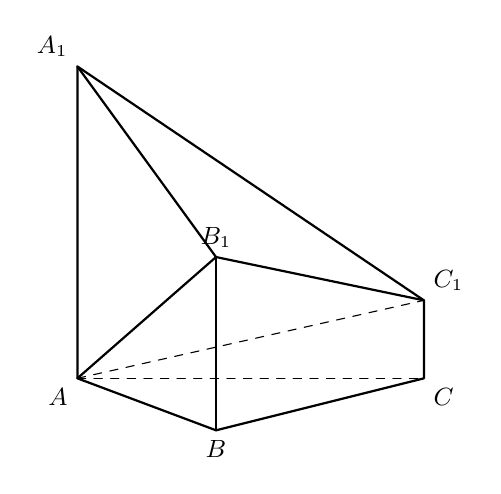
\begin{tikzpicture}[font=\small, line cap=round, line join=round, >=stealth, scale=1.1]
  % 顶点定义
  \coordinate (A) at (0, 0);
  \coordinate (B) at (1.6, -0.6);
  \coordinate (C) at (4.0, 0);
  \coordinate (A1) at (0, 3.6);
  \coordinate (B1) at (1.6, 1.4);
  \coordinate (C1) at (4.0, 0.9);

  % 虚线（隐藏棱）
  \draw[dashed, thin] (A) -- (C);
  \draw[dashed, thin] (A) -- (C1);

  % 实线（可见棱）
  \draw[thick] (A1) -- (A) -- (B) -- (C) -- (C1) -- cycle;
  \draw[thick] (B) -- (B1);
  \draw[thick] (A1) -- (B1) -- (C1);
  \draw[thick] (A) -- (B1);

  % 顶点标签
  \node[above left] at (A1) {$A_1$};
  \node[above] at (B1) {$B_1$};
  \node[above right] at (C1) {$C_1$};
  \node[below left] at (A) {$A$};
  \node[below] at (B) {$B$};
  \node[below right] at (C) {$C$};
\end{tikzpicture}
\end{center}
\nopagebreak[4]
(1) 证明：$AB_1 \perp$ 平面 $A_1B_1C_1$；
(2) 求直线 $AC_1$ 与平面 $ABB_1$ 所成的角的正弦值。

\Needspace{4\baselineskip}
\textbf{解析}

在多面体 $ABCA_1B_1C_1$ 中，$A_1A, B_1B, C_1C$ 均垂直于平面 $ABC$。
已知 $\angle ABC = 120^\circ$，$A_1A = 4$，$C_1C = 1$，$AB = BC = B_1B = 2$。

\Needspace{5\baselineskip}
\textbf{(1) 证明} 在 $\triangle ABC$ 中，由余弦定理：
\nopagebreak[4]
\[AC^2 = AB^2 + BC^2 - 2AB \cdot BC \cos 120^\circ = 4 + 4 - 2 \times 2 \times 2 \times \left(-\dfrac12\right) = 12.\]
故 $AC = 2\sqrt3$。
因为 $A_1A, B_1B, C_1C$ 均垂直于平面 $ABC$，所以各侧棱互相平行，且垂直于底面内的各线段。
\begin{itemize}
\item 在侧面 $ABB_1A_1$ 中，$A_1A \perp AB, B_1B \perp AB$，侧面为直角梯形：
\end{itemize}
\nopagebreak[4]
\[AB_1^2 = AB^2 + BB_1^2 = 2^2 + 2^2 = 8,\]
\nopagebreak[4]
\[A_1B_1^2 = (A_1A - B_1B)^2 + AB^2 = (4 - 2)^2 + 2^2 = 8.\]
  在 $\triangle AA_1B_1$ 中，$A_1A^2 = 4^2 = 16 = AB_1^2 + A_1B_1^2$。
  由勾股定理逆定理，可得 $AB_1 \perp A_1B_1$。
\begin{itemize}
\item 在侧面 $BCC_1B_1$ 中，$B_1B \perp BC, C_1C \perp BC$：
\end{itemize}
\nopagebreak[4]
\[B_1C_1^2 = (B_1B - C_1C)^2 + BC^2 = (2 - 1)^2 + 2^2 = 1 + 4 = 5.\]
\begin{itemize}
\item 在侧面 $ACC_1A_1$ 中，$A_1A \perp AC, C_1C \perp AC$：
\end{itemize}
\nopagebreak[4]
\[AC_1^2 = AC^2 + C_1C^2 = 12 + 1^2 = 13.\]
\begin{itemize}
\item 在 $\triangle AB_1C_1$ 中：
\end{itemize}
\nopagebreak[4]
\[AB_1^2 + B_1C_1^2 = 8 + 5 = 13 = AC_1^2.\]
  由勾股定理逆定理，可得 $AB_1 \perp B_1C_1$。
因为 $A_1B_1 \cap B_1C_1 = B_1$，且 $A_1B_1, B_1C_1 \subset$ 平面 $A_1B_1C_1$，
所以 $AB_1 \perp$ 平面 $A_1B_1C_1$。

\textbf{(2) 解析} 以 $B$ 为坐标原点，建立空间直角坐标系。
在底面 $ABC$ 内，以射线 $BA$ 为 $y$ 轴正方向，过 $B$ 作 $BA$ 的垂线为 $x$ 轴正方向（使点 $C$ 具有正横坐标），以射线 $BB_1$ 为 $z$ 轴正方向。
因为 $\angle ABC = 120^\circ$，所以边 $BC$ 与 $x$ 轴正向夹角为 $30^\circ$，与 $y$ 轴负向夹角为 $60^\circ$。
\Needspace{5\baselineskip}
各点坐标确定如下：
\nopagebreak[4]
\[B(0, 0, 0),\quad A(0, 2, 0),\quad B_1(0, 0, 2),\]
\nopagebreak[4]
\[C(2\cos 30^\circ, -2\sin 30^\circ, 0) = (\sqrt3, -1, 0),\]
\nopagebreak[4]
\[C_1(\sqrt3, -1, 1).\]
\Needspace{5\baselineskip}
计算向量 $\overrightarrow{AC_1}$：
\nopagebreak[4]
\[\overrightarrow{AC_1} = (\sqrt3 - 0, -1 - 2, 1 - 0) = (\sqrt3, -3, 1).\]
\Needspace{5\baselineskip}
其模长为：
\nopagebreak[4]
\[|\overrightarrow{AC_1}| = \sqrt{(\sqrt3)^2 + (-3)^2 + 1^2} = \sqrt{3 + 9 + 1} = \sqrt{13}.\]
\Needspace{5\baselineskip}
因为点 $A, B, B_1$ 均位于 $yOz$ 平面上，所以平面 $ABB_1$ 的法向量可取为：
\nopagebreak[4]
\[\boldsymbol n = (1, 0, 0).\]
\Needspace{5\baselineskip}
设直线 $AC_1$ 与平面 $ABB_1$ 所成的角为 $\theta$，则：
\nopagebreak[4]
\[\sin\theta = |\cos\langle \overrightarrow{AC_1}, \boldsymbol n\rangle| = \dfrac{|\overrightarrow{AC_1} \cdot \boldsymbol n|}{|\overrightarrow{AC_1}| |\boldsymbol n|} = \dfrac{|\sqrt3 \times 1 + 0 + 0|}{\sqrt{13} \times 1} = \dfrac{\sqrt3}{\sqrt{13}} = \dfrac{\sqrt{39}}{13}.\]
故直线 $AC_1$ 与平面 $ABB_1$ 所成角的正弦值为 $\dfrac{\sqrt{39}}{13}$。

\gkanswer{答案（1）：证明见解析版。}

\gkanswer{答案（2）：$\dfrac{\sqrt{39}}{13}$}

\end{answer}
\begin{answer}
\gksolhead{20}{}

\textbf{题目}（本小题满分 15 分）：

已知等比数列 $\{a_n\}$ 的公比 $q > 1$，且 $a_3 + a_4 + a_5 = 28$，$a_4 + 2$ 是 $a_3, a_5$ 的等差中项。数列 $\{b_n\}$ 满足 $b_1 = 1$，数列 $\{(b_{n+1} - b_n)a_n\}$ 的前 $n$ 项和为 $2n^2 + n$。
(1) 求 $q$ 的值；
(2) 求数列 $\{b_n\}$ 的通项公式。

\Needspace{4\baselineskip}
\textbf{解析}

等比数列 $\{a_n\}$ 的公比 $q > 1$。
已知 $a_3 + a_4 + a_5 = 28$，$a_4 + 2$ 是 $a_3, a_5$ 的等差中项。
数列 $\{b_n\}$ 满足 $b_1 = 1$，数列 $\{(b_{n+1} - b_n)a_n\}$ 的前 $n$ 项和为 $S_n = 2n^2 + n$。

\Needspace{5\baselineskip}
\textbf{(1) 解析} 由等差中项性质：
\nopagebreak[4]
\[a_3 + a_5 = 2(a_4 + 2) = 2a_4 + 4.\]
\Needspace{5\baselineskip}
代入 $a_3 + a_4 + a_5 = 28$：
\nopagebreak[4]
\[(2a_4 + 4) + a_4 = 28 \implies 3a_4 = 24 \implies a_4 = 8.\]
\Needspace{5\baselineskip}
从而：
\nopagebreak[4]
\[a_3 + a_5 = 28 - 8 = 20.\]
用公比 $q$ 表示：$a_3 = \dfrac{a_4}{q} = \dfrac{8}{q}$，$a_5 = a_4 q = 8q$。
\Needspace{5\baselineskip}
代入得：
\nopagebreak[4]
\[\dfrac{8}{q} + 8q = 20 \implies 8q^2 - 20q + 8 = 0 \implies 2q^2 - 5q + 2 = 0.\]
分解因式：$(2q - 1)(q - 2) = 0$。
因为 $q > 1$，所以 $q = 2$。

\textbf{(2) 解析} 由 $a_4 = 8$ 且 $q = 2$，可得首项 $a_1 = \dfrac{a_4}{q^3} = \dfrac{8}{8} = 1$。
故数列 $\{a_n\}$ 的通项公式为 $a_n = 2^{n-1}$。
设 $c_n = (b_{n+1} - b_n)a_n$，其前 $n$ 项和为 $S_n = 2n^2 + n$。
当 $n = 1$ 时，$c_1 = S_1 = 2 \times 1^2 + 1 = 3$；
\Needspace{5\baselineskip}
当 $n \geqslant 2$ 时：
\nopagebreak[4]
\[c_n = S_n - S_{n-1} = (2n^2 + n) - [2(n-1)^2 + (n-1)] = 4n - 1.\]
\Needspace{5\baselineskip}
当 $n = 1$ 时，$4 \times 1 - 1 = 3 = c_1$，故对任意 $n \geqslant 1$ 均有：
\nopagebreak[4]
\[c_n = (b_{n+1} - b_n)2^{n-1} = 4n - 1 \implies b_{n+1} - b_n = \dfrac{4n - 1}{2^{n-1}}.\]
\Needspace{5\baselineskip}
当 $n \geqslant 2$ 时，采用累加法：
\nopagebreak[4]
\[b_n = b_1 + \sum_{k=1}^{n-1} (b_{k+1} - b_k) = 1 + \sum_{k=1}^{n-1} \dfrac{4k - 1}{2^{k-1}}.\]
设 $T_{n-1} = \sum_{k=1}^{n-1} \dfrac{4k - 1}{2^{k-1}}$。
\Needspace{5\baselineskip}
展开：
\nopagebreak[4]
\[T_{n-1} = 3 + \dfrac{7}{2} + \dfrac{11}{4} + \cdots + \dfrac{4n - 5}{2^{n-2}}.\]
\Needspace{5\baselineskip}
同乘 $\dfrac12$：
\nopagebreak[4]
\[\dfrac12 T_{n-1} = \dfrac{3}{2} + \dfrac{7}{4} + \cdots + \dfrac{4n - 9}{2^{n-2}} + \dfrac{4n - 5}{2^{n-1}}.\]
\Needspace{5\baselineskip}
两式错位相减：
\nopagebreak[4]
\[\begin{aligned}
\dfrac12 T_{n-1} &= 3 + \left[\dfrac{4}{2} + \dfrac{4}{4} + \cdots + \dfrac{4}{2^{n-2}}\right] - \dfrac{4n - 5}{2^{n-1}} \\
&= 3 + \dfrac{2\left(1 - \dfrac{1}{2^{n-2}}\right)}{1 - \dfrac12} - \dfrac{4n - 5}{2^{n-1}} \\
&= 3 + 4\left(1 - \dfrac{1}{2^{n-2}}\right) - \dfrac{4n - 5}{2^{n-1}} \\
&= 7 - \dfrac{8}{2^{n-1}} - \dfrac{4n - 5}{2^{n-1}} \\
&= 7 - \dfrac{4n + 3}{2^{n-1}}.
\end{aligned}\]
\Needspace{5\baselineskip}
两端同乘 2：
\nopagebreak[4]
\[T_{n-1} = 14 - \dfrac{4n + 3}{2^{n-2}}.\]
\Needspace{5\baselineskip}
因此：
\nopagebreak[4]
\[b_n = 1 + T_{n-1} = 15 - \dfrac{4n + 3}{2^{n-2}}.\]
当 $n = 1$ 时，$b_1 = 15 - \dfrac{4 \times 1 + 3}{2^{-1}} = 15 - 14 = 1$，满足题意。
\Needspace{5\baselineskip}
故数列 $\{b_n\}$ 的通项公式为：
\nopagebreak[4]
\[b_n = 15 - \dfrac{4n + 3}{2^{n-2}}\quad (n \in \mathbf N^*).\]

\gkanswer{答案（1）：$q = 2$}

\gkanswer{答案（2）：$b_n = 15 - \dfrac{4n + 3}{2^{n-2}}$（或 $15 - \dfrac{8n + 6}{2^{n-1}}$）}

\end{answer}
\begin{answer}
\gksolhead{21}{}

\textbf{题目}（本小题满分 15 分）：

如图，已知点 $P$ 是 $y$ 轴左侧（不含 $y$ 轴）一点，抛物线 $C\colon y^2 = 4x$ 上存在不同的两点 $A, B$ 满足 $PA, PB$ 的中点均在 $C$ 上。
\nopagebreak[4]
\begin{center}% 2018 浙江卷第21题：抛物线弦中点几何图
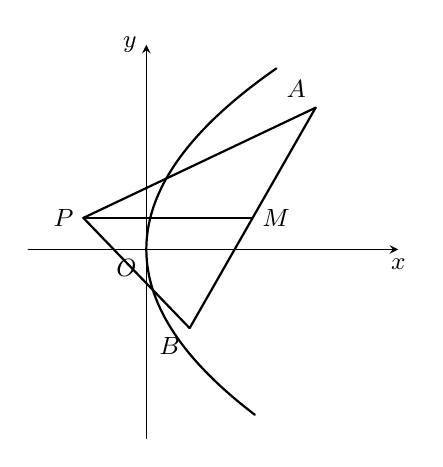
\begin{tikzpicture}[font=\small, line cap=round, line join=round, >=stealth, scale=1.0]
  % 坐标轴
  \draw[->] (-1.5, 0) -- (3.2, 0) node[below] {$x$};
  \draw[->] (0, -2.4) -- (0, 2.6) node[left] {$y$};
  \node[below left] at (0, 0) {$O$};

  % 抛物线 y^2 = 3.5x (示意)
  \draw[thick, domain=-2.1:2.3, samples=90] plot ({(\x)^2 / 3.2}, \x);

  % 关键点定义
  \coordinate (P) at (-0.8, 0.4);
  \coordinate (M) at (1.35, 0.4);
  \coordinate (A) at (2.15, 1.8);
  \coordinate (B) at (0.55, -1.0);

  % 连线
  \draw[thick] (P) -- (M);
  \draw[thick] (A) -- (B);
  \draw[thick] (P) -- (A);
  \draw[thick] (P) -- (B);

  % 标签
  \node[left] at (P) {$P$};
  \node[right] at (M) {$M$};
  \node[above left] at (A) {$A$};
  \node[below left] at (B) {$B$};
\end{tikzpicture}
\end{center}
\nopagebreak[4]
(1) 设 $AB$ 中点为 $M$，证明：$PM$ 垂直于 $y$ 轴；
(2) 若 $P$ 是半椭圆 $x^2 + \dfrac{y^2}{4} = 1\ (x < 0)$ 上的动点，求 $\triangle PAB$ 面积的取值范围。

\Needspace{4\baselineskip}
\textbf{解析}

点 $P$ 是 $y$ 轴左侧（不含 $y$ 轴）的一点，设 $P(x_0, y_0)$，其中 $x_0 < 0$。
抛物线 $C\colon y^2 = 4x$ 上存在不同的两点 $A(x_1, y_1), B(x_2, y_2)$，满足 $PA, PB$ 的中点均在抛物线 $C$ 上。

\textbf{(1) 证明} 线段 $PA$ 的中点坐标为 $\left(\dfrac{x_0 + x_1}{2}, \dfrac{y_0 + y_1}{2}\right)$。
\Needspace{5\baselineskip}
因为中点在抛物线 $y^2 = 4x$ 上，所以：
\nopagebreak[4]
\[\left(\dfrac{y_0 + y_1}{2}\right)^2 = 4 \times \dfrac{x_0 + x_1}{2} \iff (y_0 + y_1)^2 = 8(x_0 + x_1).\]
又点 $A(x_1, y_1)$ 在抛物线上，有 $y_1^2 = 4x_1 \implies 8x_1 = 2y_1^2$。
\Needspace{5\baselineskip}
代入得：
\nopagebreak[4]
\[y_0^2 + 2y_0 y_1 + y_1^2 = 8x_0 + 2y_1^2 \iff y_1^2 - 2y_0 y_1 + (8x_0 - y_0^2) = 0.\]
\Needspace{5\baselineskip}
同理，线段 $PB$ 的中点也在抛物线上，且点 $B(x_2, y_2)$ 满足抛物线方程，故 $y_2$ 也满足该方程：
\nopagebreak[4]
\[y_2^2 - 2y_0 y_2 + (8x_0 - y_0^2) = 0.\]
因为 $A, B$ 是抛物线上不同的两点，所以 $y_1, y_2$ 是一元二次方程 $y^2 - 2y_0 y + (8x_0 - y_0^2) = 0$ 的两个不同实根。
\Needspace{5\baselineskip}
判别式为：
\nopagebreak[4]
\[\Delta = (-2y_0)^2 - 4(8x_0 - y_0^2) = 8y_0^2 - 32x_0 = 8(y_0^2 - 4x_0) > 0\ (\text{\text{因} } x_0 < 0).\]
\Needspace{5\baselineskip}
由韦达定理：
\nopagebreak[4]
\[y_1 + y_2 = 2y_0,\quad y_1 y_2 = 8x_0 - y_0^2.\]
\Needspace{5\baselineskip}
设线段 $AB$ 的中点为 $M(x_M, y_M)$，则：
\nopagebreak[4]
\[y_M = \dfrac{y_1 + y_2}{2} = \dfrac{2y_0}{2} = y_0.\]
这表明点 $M$ 的纵坐标等于点 $P$ 的纵坐标，因此直线 $PM$ 与 $x$ 轴平行，即 $PM$ 垂直于 $y$ 轴。

\textbf{(2) 解析} 由 (1) 知直线 $PM$ 处于水平方向，方程为 $y = y_0$。
\Needspace{5\baselineskip}
点 $M$ 的横坐标为：
\nopagebreak[4]
\[x_M = \dfrac{x_1 + x_2}{2} = \dfrac{y_1^2 + y_2^2}{8} = \dfrac{(y_1 + y_2)^2 - 2y_1 y_2}{8} = \dfrac{4y_0^2 - 2(8x_0 - y_0^2)}{8} = \dfrac34 y_0^2 - 2x_0.\]
\Needspace{5\baselineskip}
线段 $PM$ 的长度为：
\nopagebreak[4]
\[|PM| = x_M - x_0 = \left(\dfrac34 y_0^2 - 2x_0\right) - x_0 = \dfrac34 y_0^2 - 3x_0 = 3\left(\dfrac{y_0^2}{4} - x_0\right).\]
\Needspace{5\baselineskip}
又因为 $M$ 是 $AB$ 中点，直线 $PM$ 为水平线，$\triangle PAB$ 可按 $PM$ 分割为上下两个三角形：
\nopagebreak[4]
\[\begin{aligned}
S_{\triangle PAB} &= S_{\triangle PAM} + S_{\triangle PBM} \\
&= \dfrac12 |PM| |y_1 - y_0| + \dfrac12 |PM| |y_2 - y_0| \\
&= \dfrac12 |PM| (|y_1 - y_0| + |y_2 - y_0|).
\end{aligned}\]
由于 $y_0 = \dfrac{y_1 + y_2}{2}$ 介于 $y_1$ 与 $y_2$ 之间，因此 $|y_1 - y_0| + |y_2 - y_0| = |y_1 - y_2|$。
\Needspace{5\baselineskip}
故：
\nopagebreak[4]
\[S_{\triangle PAB} = \dfrac12 |PM| |y_1 - y_2|.\]
\Needspace{5\baselineskip}
利用根与系数的关系：
\nopagebreak[4]
\[|y_1 - y_2| = \sqrt{(y_1 + y_2)^2 - 4y_1 y_2} = \sqrt{8(y_0^2 - 4x_0)} = 4\sqrt2 \sqrt{\dfrac{y_0^2}{4} - x_0}.\]
\Needspace{5\baselineskip}
代入面积公式：
\nopagebreak[4]
\[S_{\triangle PAB} = \dfrac12 \times 3\left(\dfrac{y_0^2}{4} - x_0\right) \times 4\sqrt2 \sqrt{\dfrac{y_0^2}{4} - x_0} = 6\sqrt2 \left(\dfrac{y_0^2}{4} - x_0\right)^{3/2}.\]
已知点 $P(x_0, y_0)$ 在半椭圆 $x^2 + \dfrac{y^2}{4} = 1\ (x < 0)$ 上，
所以 $\dfrac{y_0^2}{4} = 1 - x_0^2$，其中 $x_0 \in [-1, 0)$。
\Needspace{5\baselineskip}
记函数：
\nopagebreak[4]
\[t(x_0) = \dfrac{y_0^2}{4} - x_0 = 1 - x_0^2 - x_0 = -\left(x_0 + \dfrac12\right)^2 + \dfrac54.\]
在区间 $[-1, 0)$ 上：
\begin{itemize}
\item 当 $x_0 = -\dfrac12$ 时，$t(x_0)$ 取得最大值 $t_{\max} = \dfrac54$；
\item 当 $x_0 = -1$ 时，$t(-1) = 1 - (-1)^2 - (-1) = 1$；
\item 当 $x_0 \to 0^-$ 时，$t(x_0) \to 1$。
\end{itemize}
因此 $t(x_0)$ 的取值范围是闭区间 $\left[1, \dfrac54\right]$。
从而面积 $S_{\triangle PAB}$ 的取值范围为：
\begin{itemize}
\item 最小值为 $S_{\min} = 6\sqrt2 \times 1^{3/2} = 6\sqrt2$；
\item 最大值为 $S_{\max} = 6\sqrt2 \times \left(\dfrac54\right)^{3/2} = 6\sqrt2 \times \dfrac{5\sqrt5}{8} = \dfrac{15\sqrt{10}}{4}$。
\end{itemize}
故 $\triangle PAB$ 面积的取值范围为 $\left[6\sqrt2, \dfrac{15\sqrt{10}}{4}\right]$。

\gkanswer{答案（1）：证明见解析版。}

\gkanswer{答案（2）：$\left[6\sqrt2, \dfrac{15\sqrt{10}}{4}\right]$}

\end{answer}
\begin{answer}
\gksolhead{22}{}

\textbf{题目}（本小题满分 15 分）：

已知函数 $f(x) = \sqrt x - \ln x$。
(1) 若 $f(x)$ 在 $x = x_1, x_2\ (x_1 \neq x_2)$ 处导数相等，证明：$f(x_1) + f(x_2) > 8 - 8\ln 2$；
(2) 若 $a \leqslant 3 - 4\ln 2$，证明：对于任意 $k > 0$，直线 $y = kx + a$ 与曲线 $y = f(x)$ 有唯一公共点。

\Needspace{4\baselineskip}
\textbf{解析}

已知函数 $f(x) = \sqrt x - \ln x$，定义域为 $(0, +\infty)$。
\Needspace{5\baselineskip}
求导得：
\nopagebreak[4]
\[f'(x) = \dfrac{1}{2\sqrt x} - \dfrac{1}{x} = \dfrac{\sqrt x - 2}{2x}.\]

\textbf{(1) 证明} 设 $u = \sqrt{x_1}$，$v = \sqrt{x_2}$。不妨设 $0 < u < v$。
\Needspace{5\baselineskip}
由 $f'(x_1) = f'(x_2)$ 得：
\nopagebreak[4]
\[\dfrac{u - 2}{2u^2} = \dfrac{v - 2}{2v^2} \iff v^2(u - 2) = u^2(v - 2).\]
\Needspace{5\baselineskip}
展开整理：
\nopagebreak[4]
\[uv(v - u) = 2(v^2 - u^2) = 2(v - u)(u + v).\]
\Needspace{5\baselineskip}
因为 $0 < u < v$，两边同除以 $v - u > 0$：
\nopagebreak[4]
\[uv = 2(u + v) \iff \dfrac{1}{u} + \dfrac{1}{v} = \dfrac12.\]
\Needspace{5\baselineskip}
由基本不等式，由于 $u \neq v$：
\nopagebreak[4]
\[uv = 2(u + v) > 2 \times 2\sqrt{uv} = 4\sqrt{uv} \implies \sqrt{uv} > 4 \implies uv > 16.\]
且 $u + v = \dfrac{uv}{2} > 8$。
\Needspace{5\baselineskip}
计算 $f(x_1) + f(x_2)$：
\nopagebreak[4]
\[\begin{aligned}
f(x_1) + f(x_2) &= (\sqrt{x_1} - \ln x_1) + (\sqrt{x_2} - \ln x_2) \\
&= u - 2\ln u + v - 2\ln v \\
&= (u + v) - 2\ln(uv) \\
&= \dfrac{uv}{2} - 2\ln(uv).
\end{aligned}\]
设 $t = \sqrt{uv}$，由上可知 $t > 4$，$uv = t^2$。
构造函数 $g(t) = \dfrac{t^2}{2} - 4\ln t\ (t > 4)$。
\Needspace{5\baselineskip}
求导：
\nopagebreak[4]
\[g'(t) = t - \dfrac{4}{t} = \dfrac{t^2 - 4}{t}.\]
当 $t > 4$ 时，$t^2 > 16 > 4$，故 $g'(t) > 0$ 恒成立。
因此 $g(t)$ 在 $(4, +\infty)$ 上严格单调递增。
\Needspace{5\baselineskip}
所以：
\nopagebreak[4]
\[g(t) > g(4) = \dfrac{4^2}{2} - 4\ln 4 = 8 - 8\ln 2.\]
即 $f(x_1) + f(x_2) > 8 - 8\ln 2$ 得证。

\textbf{(2) 证明} 直线与曲线的公共点横坐标即为方程 $f(x) - (kx + a) = 0$ 在 $(0, +\infty)$ 上的实根。
\Needspace{5\baselineskip}
构造辅助函数：
\nopagebreak[4]
\[h(x) = \sqrt x - \ln x - kx - a\quad (x > 0).\]
\Needspace{5\baselineskip}
求导：
\nopagebreak[4]
\[h'(x) = \dfrac{1}{2\sqrt x} - \dfrac{1}{x} - k = \dfrac{\sqrt x - 2 - 2kx}{2x}.\]
令 $u = \sqrt x > 0$，设分子二次函数为 $\varphi(u) = -2ku^2 + u - 2$。
\Needspace{5\baselineskip}
二次函数 $\varphi(u)$ 开口向下，判别式为：
\nopagebreak[4]
\[\Delta = 1^2 - 4(-2k)(-2) = 1 - 16k.\]
分以下两种情形讨论：
1. \textbf{情形一：$k \geqslant \dfrac{1}{16}$}：
   此时 $\Delta \leqslant 0$，对任意 $u > 0$ 均有 $\varphi(u) \leqslant 0$（仅当 $k = \dfrac{1}{16}, u = 4$ 时取得 $0$）。
   因此 $h'(x) \leqslant 0$ 在 $(0, +\infty)$ 上恒成立，且仅在孤立点处导数为 0。
   所以 $h(x)$ 在 $(0, +\infty)$ 上严格单调递减。
\Needspace{5\baselineskip}
   又因为：
\nopagebreak[4]
\[\lim_{x \to 0^+} h(x) = +\infty,\quad \lim_{x \to +\infty} h(x) = -\infty,\]
   根据零点存在定理与单调性，函数 $h(x)$ 在 $(0, +\infty)$ 上存在唯一的零点。
2. \textbf{情形二：$0 < k < \dfrac{1}{16}$}：
   此时 $\Delta = 1 - 16k > 0$。
\Needspace{5\baselineskip}
   方程 $-2ku^2 + u - 2 = 0$ 有两个不同的正实根：
\nopagebreak[4]
\[u_1 = \dfrac{1 - \sqrt{1 - 16k}}{4k} = \dfrac{4}{1 + \sqrt{1 - 16k}},\quad u_2 = \dfrac{1 + \sqrt{1 - 16k}}{4k}.\]
\Needspace{5\baselineskip}
   因为 $0 < \sqrt{1 - 16k} < 1$，所以：
\nopagebreak[4]
\[2 < u_1 < 4 < u_2.\]
   设 $x_1 = u_1^2$，$x_2 = u_2^2$，满足 $0 < x_1 < x_2$。
   在区间 $(0, x_1)$ 上，$\varphi(u) < 0 \implies h'(x) < 0$，$h(x)$ 单调递减；
   在区间 $(x_1, x_2)$ 上，$\varphi(u) > 0 \implies h'(x) > 0$，$h(x)$ 单调递增；
   在区间 $(x_2, +\infty)$ 上，$\varphi(u) < 0 \implies h'(x) < 0$，$h(x)$ 单调递减。
   因此，$x_1$ 是极小值点，$x_2$ 是极大值点。
\Needspace{5\baselineskip}
   在极小值点 $x_1$ 处，有 $h'(x_1) = 0$，即：
\nopagebreak[4]
\[\dfrac{\sqrt{x_1} - 2}{2x_1} = k \implies kx_1 = \dfrac{\sqrt{x_1} - 2}{2} = \dfrac{u_1 - 2}{2}.\]
\Needspace{5\baselineskip}
   将 $kx_1$ 代入极小值 $h(x_1)$：
\nopagebreak[4]
\[\begin{aligned}
h(x_1) &= \sqrt{x_1} - \ln x_1 - kx_1 - a \\
&= u_1 - 2\ln u_1 - \dfrac{u_1 - 2}{2} - a \\
&= \dfrac{u_1 + 2}{2} - 2\ln u_1 - a.
\end{aligned}\]
\Needspace{5\baselineskip}
   考察函数 $\psi(u) = \dfrac{u + 2}{2} - 2\ln u$ 在区间 $(2, 4)$ 上的性质：
\nopagebreak[4]
\[\psi'(u) = \dfrac12 - \dfrac{2}{u} = \dfrac{u - 4}{2u}.\]
   当 $u \in (2, 4)$ 时，$\psi'(u) < 0$，所以 $\psi(u)$ 在 $(2, 4)$ 上单调严格递减。
\Needspace{5\baselineskip}
   因为 $u_1 \in (2, 4)$，所以：
\nopagebreak[4]
\[\psi(u_1) > \psi(4) = \dfrac{4 + 2}{2} - 2\ln 4 = 3 - 4\ln 2.\]
\Needspace{5\baselineskip}
   已知 $a \leqslant 3 - 4\ln 2$，故：
\nopagebreak[4]
\[h(x_1) = \psi(u_1) - a > (3 - 4\ln 2) - a \geqslant 0.\]
   由于 $h(x_1) > 0$ 为函数在 $(0, x_2]$ 上的极小值，所以：
   对任意 $x \in (0, x_2]$，均有 $h(x) \geqslant h(x_1) > 0$，函数在 $(0, x_2]$ 上无零点。
   而在区间 $[x_2, +\infty)$ 上：
   $h(x_2) > h(x_1) > 0$，$h(x)$ 连续且严格单调递减，且 $\lim\limits_{x \to +\infty} h(x) = -\infty$。
   由零点存在定理和单调性，函数 $h(x)$ 在 $[x_2, +\infty)$ 上有且仅有 1 个零点。
综合情形一与情形二，当 $a \leqslant 3 - 4\ln 2$ 时，对于任意 $k > 0$，方程 $f(x) - (kx + a) = 0$ 在 $(0, +\infty)$ 上有且仅有 1 个实根，即直线 $y = kx + a$ 与曲线 $y = f(x)$ 有唯一公共点。
命题得证。

\gkanswer{答案（1）：证明见解析版。}

\gkanswer{答案（2）：证明见解析版。}

\end{answer}